
\chapter{搜索工程和算法架构体系} 
\thispagestyle{empty}

\setlength{\fboxrule}{0pt}\setlength{\fboxsep}{0cm}
\noindent\shadowbox{
\begin{tcolorbox}[arc=0mm,colback=lightblue,colframe=darkblue,title=学习目标与要求]
%\kai\textcolor{darkblue}{1.~~.} \\ 

\end{tcolorbox}}
\setlength{\fboxrule}{1pt}\setlength{\fboxsep}{4pt} 

\section{工程架构} 

\begin{figure}[h]
\centering
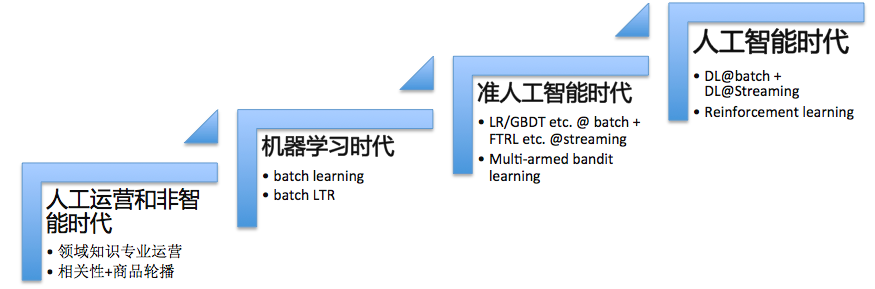
\includegraphics[totalheight=2.5in]{fig/searchAlgoRoadmap.png}
\caption{工程架构图} \label{fig:gansamples}
\end{figure}

\section{算法架构} 

大规模机器学习体系如下图所示:
\begin{figure}[h]
\centering
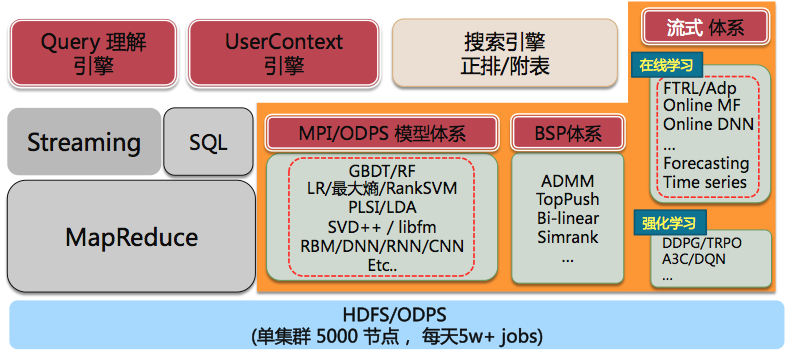
\includegraphics[totalheight=2.5in]{fig/searchAlgoArch.png}
\caption{大规模机器学习@淘宝搜索} \label{fig:gansamples}
\end{figure}

\section{评估指标及ab系统} 
我们平台上所关心的指标有: 
\begin{description} 
	\item uv转化率: $ cvr=\frac{buyuv}{uv} $
	\item uv点击率: $ ctr=\frac{ipvuv}{uv} $
	\item 客单价: 
	\item GMV:
\end{description}

\section{工作流和数据流} 



\begin{thebibliography}{99}
\addcontentsline{toc}{chapter}{\protect\numberline{}{\hspace{-1.5em}参考文献}}
\markboth{参考文献}{参考文献}
\bibitem{1} C. Burges, T. Shaked, etc.., Learning to rank 
using gradient descent. In Proceedings of the 22nd international 
conference on machine learning, ACM
\end{thebibliography}

 
